
\chapter{System resolution}
\section{Properties of the stiffness matrix}
	We have the assembly, the BC are applied, we are ready to solve the system: $Kq = f$. K is a symmetric matrix since:
	
	\begin{equation}
	K = \int _{V} B^T HB \, dV
	\end{equation}
	
	where H is symmetric. K is positive definite after application of BC, the strain energy if $q$ is non-zero is:
	
	\begin{equation}
	W = \frac{1}{2} q^T K q >  0. 
	\end{equation}
	
	\wrapfig{8}{l}{7}{0.3}{ch11/1}
	Finally K is \textbf{sparse}, this means that the non-zero terms appear where the degrees of freedom are connected. The matrix is concentrated around the \textbf{bandwisth}, the narrowest zone parallel to the main diagonal for which all the terms vanish outside this zone. In addition, K is assumed to be of order n, full rank, invertible and non-singular. It is important for the matrix to be sparse, so that we significantly decrease the computation time! 
	
\section{Algorithms for solving linear systems}
	\wrapfig{8}{r}{7}{0.3}{ch11/2}
	The main approaches are summarized on the figure. Direct methods are based on the bandwidth or the \textbf{frontwidth} which consists in progressing through the domain by Gauss elimination. 
	
\subsection{Direct methods}
	It is composed of a single large step, works for any invertible matrix and provides the exact solution. Costly operations: $O_{2D}(n^2), O_{3D}(n^{7/3})$, and high memory usage. But it is faster for small matrices. It destroy the sparsity of the initial matrix. The Gauss elimination is used, we extract one unknown in function of the others and replace it in other equations to get a n-1 matrix, and we repeat this process till finding one unknown. The process is then repeated backward to compute all the unknowns. LU decomposition is represented in the next slides: 
	
	\minifig{ch11/3}{ch11/4}{0.15}{0.15}{0.45}{0.45}
	\minifig{ch11/5}{ch11/6}{0.15}{0.15}{0.45}{0.45}
	\minifig{ch11/7}{ch11/8}{0.15}{0.15}{0.45}{0.45}
	
\subsection{Cholesky decomposition}
	\wrapfig{3}{l}{7}{0.15}{ch11/9}
	The previous method being costly, it is obvious to take advantage of the symmetry of K. The new method is summarized on the slide. 
	
	\newpage
\subsection{Frontal method}
	This consists in never assembling the stiffness matrix: 
	\minifig{ch11/10}{ch11/11}{0.15}{0.15}{0.45}{0.45}
	\minifig{ch11/12}{ch11/13}{0.15}{0.15}{0.45}{0.45}
	
\subsection{Iterative methods}
	The method consists in, starting from an initial guess, finding successive approximations. Preconditionners determine the efficiency of the method. The total computational work is not known as the iteration number is not known, but the work evolution is less high. Memory storage grows linearly, well adapted for very large scale problems. The problem is not solved exactly but we have a convergence. 
	
	\minifig{ch11/14}{ch11/15}{0.15}{0.15}{0.45}{0.45}
	\minifig{ch11/16}{ch11/17}{0.15}{0.15}{0.45}{0.45}
	
	\begin{center}
	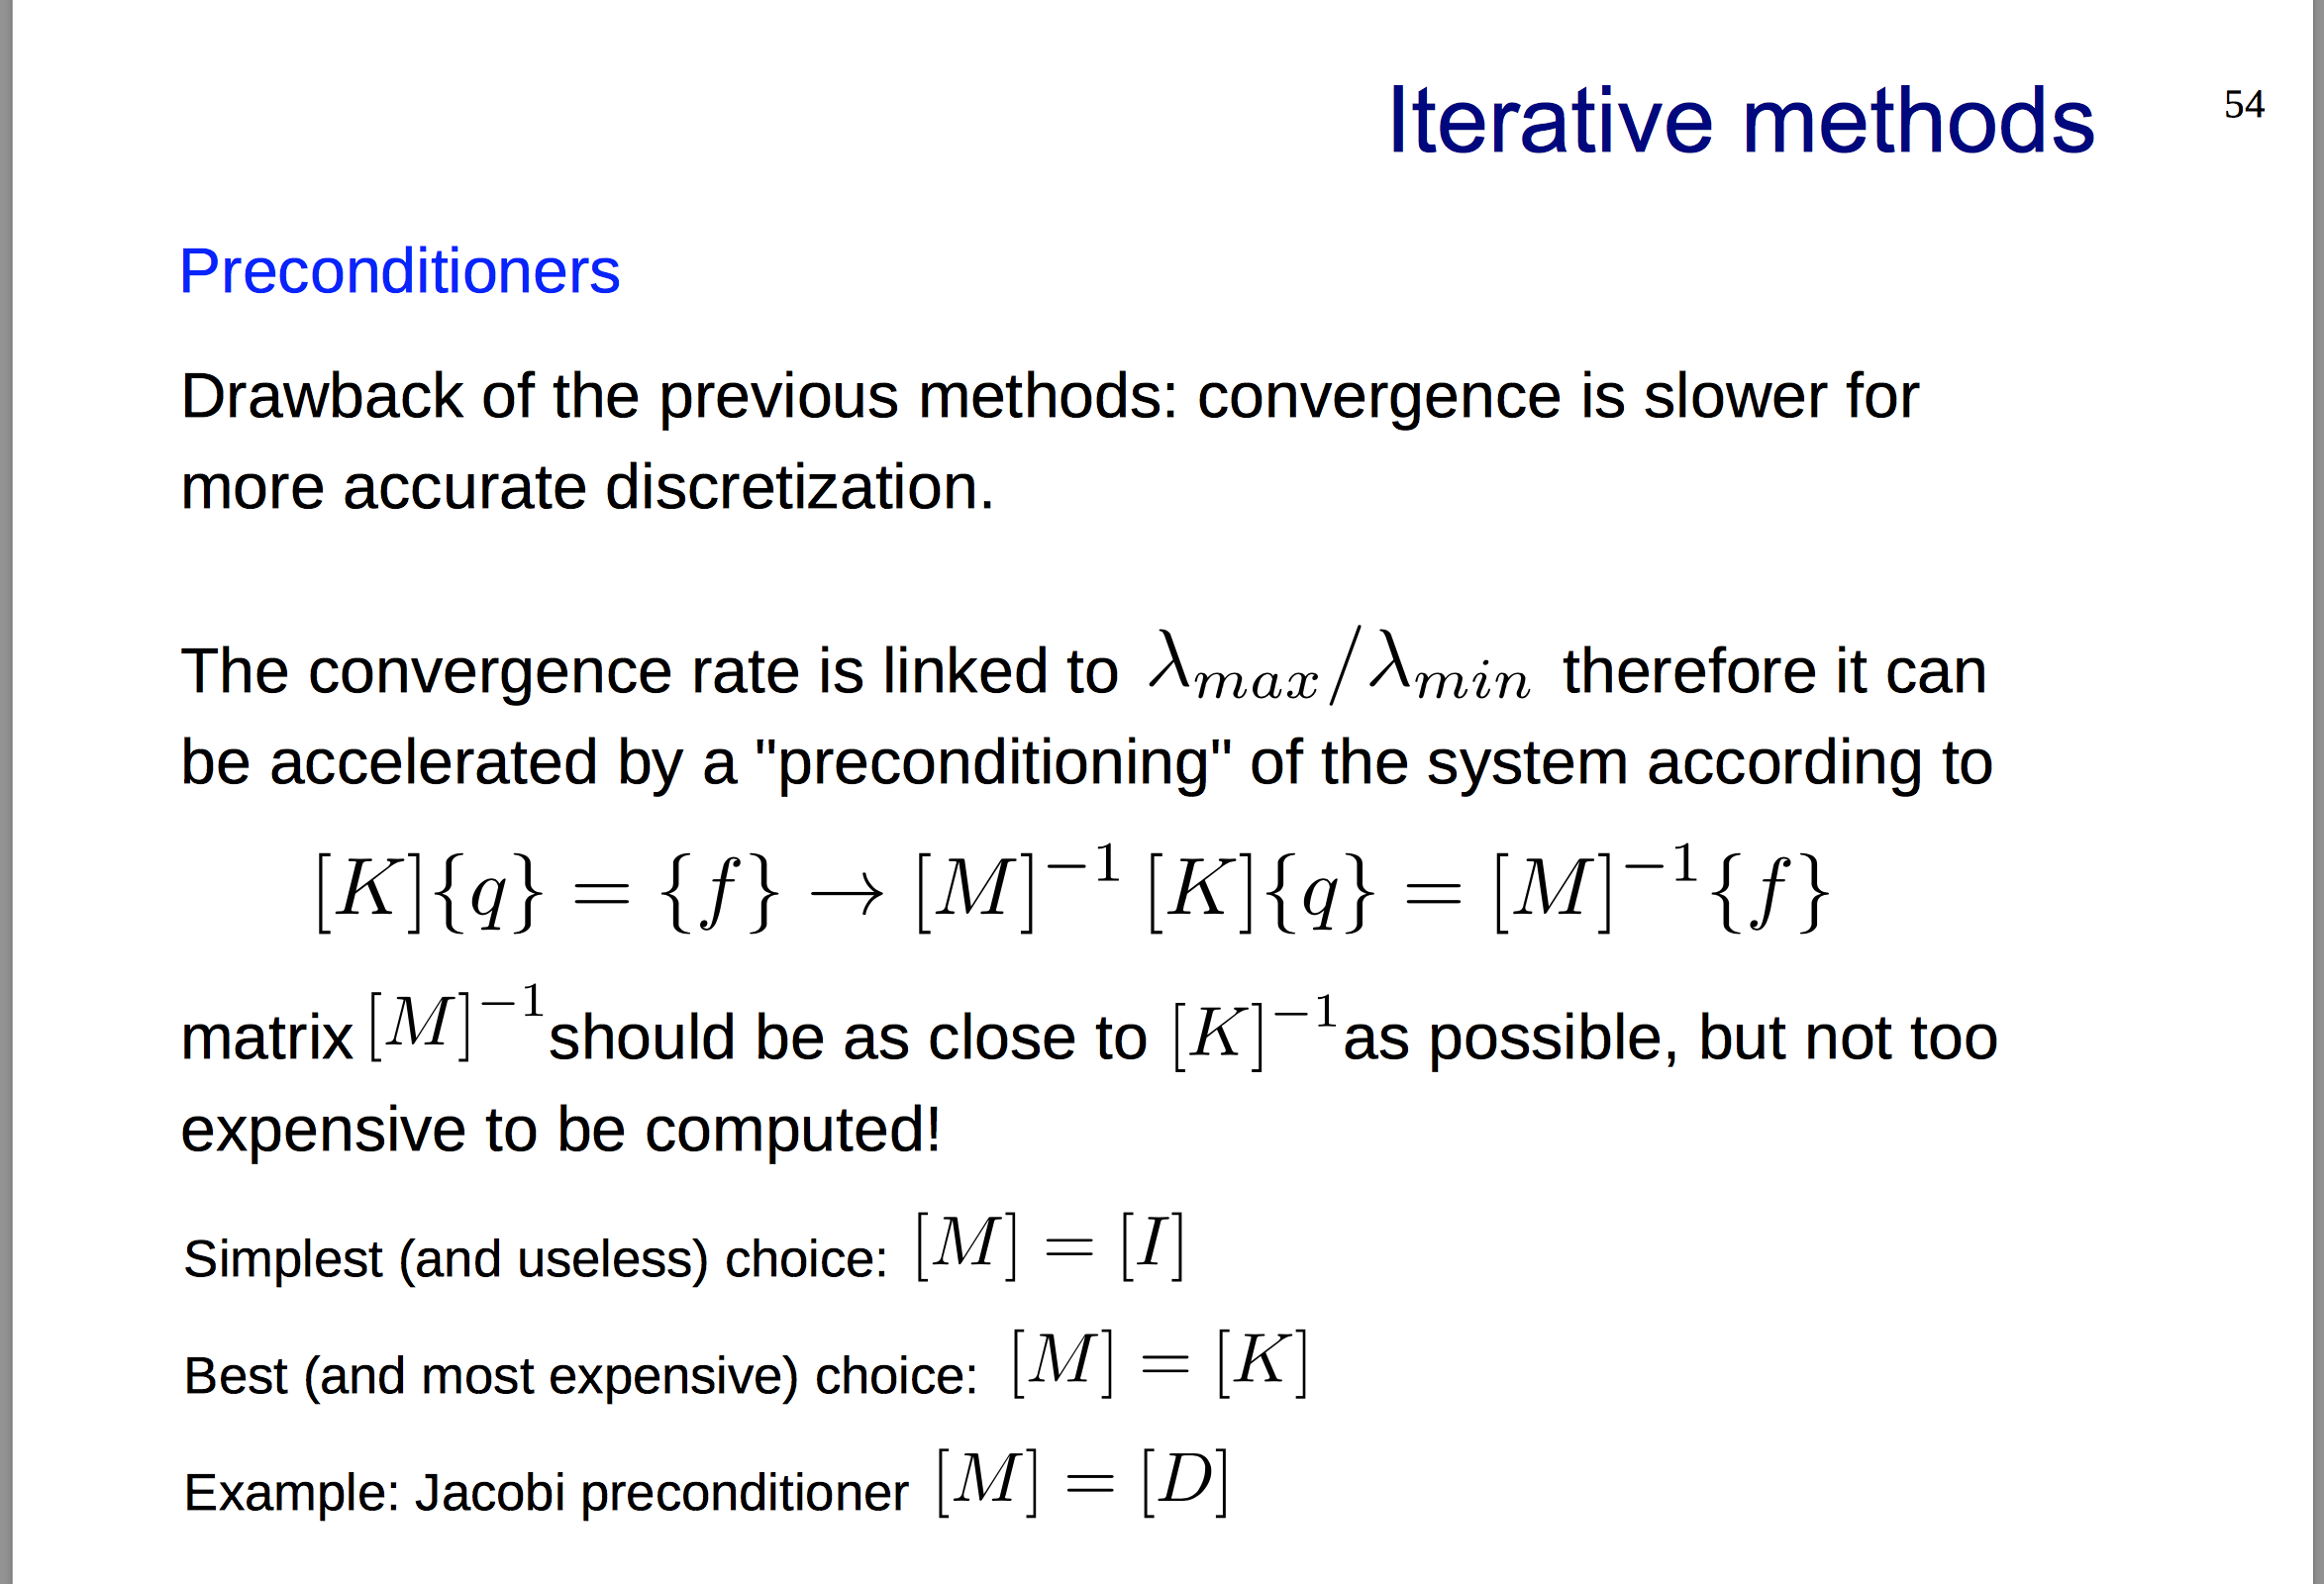
\includegraphics[scale=0.15]{ch11/18}
	\captionof{figure}{}
	\end{center}
	